\documentclass[11pt]{article}
\usepackage[margin=1in]{geometry}
\usepackage{amsmath,amssymb}
\usepackage{booktabs}
\usepackage{graphicx}
\usepackage{url}
\usepackage{listings}
\usepackage{xcolor}
\providecommand{\citep}{\cite}
\providecommand{\citet}{\cite}
\lstset{basicstyle=\ttfamily\small, breaklines=true, frame=single,
  backgroundcolor=\color{gray!10}}

\title{Supplementary Material\\[0.4em]
\large Evaluating Tool-Using Language Agents: Judge Reliability,
Propagation Cascades, and Runtime Mitigation in AgentProp-Bench}
\date{}

\begin{document}
\maketitle
\tableofcontents
\newpage

\section{Code, Data, and Trace Availability}
All code, data, agent traces, and human labels are public at
\url{https://github.com/bhaskargurram-ai/agenthallu-bench}.
The repository contains: \texttt{data/results/} (result CSVs and analysis
JSONs, including per-open-model baseline/P2 and ensemble re-judgements),
\texttt{data/tasks/} (2{,}000 task specifications), \texttt{experiments/}
(runners), \texttt{analysis/} (statistics, merge, tool-call-rate scripts),
\texttt{metrics/} (EPS scorer, cascade detector), \texttt{agent/} (ReAct agent,
model router with the local vLLM backend, tool executor),
\texttt{benchmark/} (task generator and four domain simulators),
\texttt{interceptor/}, and \texttt{tests/}. The command
\texttt{bash analysis/finalize\_openmodels.sh} regenerates every table and
figure and recompiles the manuscript.

\section{Open-Weight Model Serving and Tool-Call Adherence}
Open-weight models were served locally with vLLM through an OpenAI-compatible
endpoint and driven by the \emph{same} prompted-ReAct harness as the
proprietary models (the injection acts on the parsed tool call, which is
model-agnostic). Table~\ref{tab:toolcallS} reports the tool-call rate---the
fraction of P2 semantic-wrong traces containing a parseable tool call---for
every model evaluated. Only models that reliably emit tool calls yield
measurable propagation; Mistral-7B-Instruct-v0.2 and Phi-3.5-mini did not and
are therefore excluded from the propagation tables.

\begin{table}[h]
\centering
\caption{Tool-call rate and fabricated-tool-use rate on P2 semantic-wrong
traces. Fabricated tool use = no tool call emitted, yet the final answer
asserts a completed tool-derived result.}
\label{tab:toolcallS}
\begin{tabular}{llrr}
\toprule
Model & Type & Tool-call rate & Fabricated \\
\midrule
GPT-4o            & proprietary & 100.0\% & 0.0\% \\
GPT-4.1-nano      & proprietary & 99.0\%  & 0.5\% \\
o3-mini           & proprietary & 88.0\%  & 8.0\% \\
DeepSeek-V3       & proprietary & 86.0\%  & 7.0\% \\
GPT-4.1-mini      & proprietary & 85.0\%  & 12.0\% \\
Gemini-2.5-Flash  & proprietary & 76.0\%  & 18.0\% \\
GPT-3.5-Turbo     & proprietary & 59.5\%  & 21.5\% \\
GPT-4o-mini       & proprietary & 40.0\%  & 24.0\% \\
Gemini-2.0-Flash  & proprietary & 5.0\%   & 42.5\% \\
\midrule
Qwen2.5-7B        & open-weight & 99.5\%  & --- \\
Qwen2.5-3B        & open-weight & 70.0\%  & --- \\
Qwen2.5-14B       & open-weight & 61.0\%  & --- \\
Hermes-3-Llama-3.1-8B & open-weight & 37.0\% & --- \\
Mistral-7B-v0.2   & open-weight & 21.5\%  & --- \\
Phi-3.5-mini      & open-weight & 0.0\%   & --- \\
\bottomrule
\end{tabular}
\end{table}

\section{Interceptor Threshold Sweep}
Table~\ref{tab:sweep} reports the 12-configuration sweep on the validation
split ($n{=}40$ P2 rows). The reported $F_1{=}0.842$ is a sweep-internal
optimum, not a held-out estimate.
% Source: analysis/interceptor_tuned_thresholds.json
\begin{table}[t]
\centering
\caption{Full interceptor threshold sweep. Each row is a configuration of the three-layer filter: L1 (tool-call repetition threshold), L2 (keyword match count), L3 (LLM self-check). Best configuration by $F_1$ is highlighted. $N = 960$ P2 sessions.}
\label{tab:sweep}
\begin{tabular}{r r c r r r r}
\toprule
L1 thresh & L2 kw & L3 & $F_1$ & Precision & Recall & Abstain\% \\
\midrule
1 & 2 & \checkmark & 0.842 $\star$ & 0.923 & 0.774 & 65.0 \\
1 & 2 & --- & 0.809 & 0.826 & 0.792 & 57.5 \\
1 & 3 & \checkmark & 0.808 & 0.955 & 0.700 & 55.0 \\
1 & 3 & --- & 0.776 & 0.826 & 0.731 & 57.5 \\
2 & 2 & \checkmark & 0.762 & 0.842 & 0.696 & 47.5 \\
2 & 2 & --- & 0.780 & 0.889 & 0.696 & 45.0 \\
2 & 3 & \checkmark & 0.810 & 0.850 & 0.773 & 50.0 \\
2 & 3 & --- & 0.833 & 0.938 & 0.750 & 40.0 \\
3 & 2 & \checkmark & 0.769 & 0.938 & 0.652 & 40.0 \\
3 & 2 & --- & 0.750 & 0.857 & 0.667 & 35.0 \\
3 & 3 & \checkmark & 0.667 & 0.824 & 0.560 & 42.5 \\
3 & 3 & --- & 0.800 & 0.933 & 0.700 & 37.5 \\
\bottomrule
\end{tabular}
\end{table}

\section{Self-Consistency Baseline ($k{=}3$)}
Table~\ref{tab:selfconsistency} reports $k{=}3$ self-consistency voting on 30 tasks per
condition; at $n{=}30$ this comparison is directional only.
% Source: data/results/self_consistency_results.csv
\begin{table}[t]
\centering
\caption{Self-consistency analysis ($k = 3$ runs per task). Unique answers is the median count of distinct answers across repetitions. Hallucination rate is measured by heuristic match. Conditions: baseline (no injection) vs.\ P2 (semantic-wrong injection).}
\label{tab:selfconsistency}
\begin{tabular}{l l r r r r}
\toprule
Model & Condition & $n$ & Halluc.\% & Median uniq.\ ans. & Abstain\% \\
\midrule
DeepSeek-V3 & baseline & 30 & 30.0 & 2.0 & 46.7 \\
DeepSeek-V3 & p2_semantic & 30 & 23.3 & 3.0 & 60.0 \\
\midrule
GPT-4o-mini & baseline & 30 & 20.0 & 3.0 & 70.0 \\
GPT-4o-mini & p2_semantic & 30 & 23.3 & 3.0 & 56.7 \\
\bottomrule
\end{tabular}
\end{table}

\section{Cross-Domain Replication: Retail}
Table~\ref{tab:retail} reports baseline correctness and mean EPS on the 300
held-out retail tasks.
% Source: data/results/baseline_retail.csv, data/results/p2_retail.csv
\begin{table}[t]
\centering
\caption{Cross-domain transfer: held-out retail tasks. Models were not exposed to retail tasks during P2 tuning. Correctness judged by heuristic match. 95\% bootstrap CIs ($B = 1{,}000$).}
\label{tab:retail}
\begin{tabular}{l r r l r r l}
\toprule
Model & $n_{\mathrm{BL}}$ & BL\% & CI & $n_{\mathrm{P2}}$ & P2\% & CI \\
\midrule
DeepSeek-V3 & 100 & 37.0 & [27.0, 47.0] & 100 & 43.0 & [33.0, 53.0] \\
GPT-4o-mini & 100 & 29.0 & [20.0, 38.0] & 100 & 33.0 & [24.0, 42.0] \\
Gemini-2.0-Flash & 100 & 17.0 & [10.0, 25.0] & 100 & 17.0 & [10.0, 25.0] \\
\bottomrule
\end{tabular}
\end{table}

\section{Interceptor Layer Ablation}
Table~\ref{tab:ablation} ablates the interceptor layers on GPT-4o-mini.
% Source: data/results/ablation_results.csv
\begin{table}[t]
\centering
\caption{Interceptor ablation study. Each condition removes one layer of the three-layer interceptor. Hallucination rate and abstain rate are reported. 95\% bootstrap CIs ($B = 1{,}000$).}
\label{tab:ablation}
\begin{tabular}{l l r r r r}
\toprule
Model & Condition & $n$ & Halluc.\% & Abstain\% & Correct\% \\
\midrule
Gemini-2.0-Flash & l1_l2 & 60 & 51.7 & 0.0 & 48.3 \\
Gemini-2.0-Flash & l1_l2_l3 & 60 & 48.3 & 1.7 & 50.0 \\
Gemini-2.0-Flash & l1_only & 60 & 48.3 & 0.0 & 51.7 \\
\midrule
GPT-4o-mini & l1_l2 & 60 & 46.7 & 11.7 & 41.7 \\
GPT-4o-mini & l1_l2_l3 & 60 & 41.7 & 26.7 & 31.7 \\
GPT-4o-mini & l1_only & 60 & 51.7 & 18.3 & 30.0 \\
\bottomrule
\end{tabular}
\end{table}

\section{Power Analysis}
Table~\ref{tab:power} reports Cohen's $h$ and achieved power for each
statistical claim.
% Source: recomputed from baseline_all.csv, p2_all_rejudged.csv, interceptor CSVs
\begin{table}[t]
\centering
\caption{Post-hoc power analysis for all main contrasts. Effect size is Cohen's $h$; achieved power is computed at $\alpha = 0.05$ (two-sided). Contrasts with power $< 0.80$ are flagged (\dag).}
\label{tab:power}
\small
\begin{tabular}{l r r r r r r}
\toprule
Contrast & $n_1$ & $n_2$ & $p_1$ & $p_2$ & $h$ & Power \\
\midrule
DeepSeek-V3: P2 vs BL & 450 & 200 & 0.482 & 0.625 & 0.288 & 0.924 \\
GPT-3.5-Turbo: P2 vs BL & 450 & 200 & 0.496 & 0.675 & 0.366 & 0.991 \\
GPT-4.1-mini: P2 vs BL & 450 & 200 & 0.453 & 0.655 & 0.409 & 0.998 \\
GPT-4.1-nano: P2 vs BL & 450 & 200 & 0.547 & 0.845 & 0.668 & 1.000 \\
GPT-4o-mini: P2 vs BL & 450 & 200 & 0.600 & 0.710 & 0.232 & 0.780$^{\dag}$ \\
Gemini-2.0-Flash: P2 vs BL & 450 & 200 & 0.524 & 0.670 & 0.298 & 0.939 \\
Qwen2.5-14B: P2 vs BL & 450 & 200 & 0.444 & 0.625 & 0.364 & 0.990 \\
Qwen2.5-3B: P2 vs BL & 450 & 200 & 0.458 & 0.825 & 0.792 & 1.000 \\
Qwen2.5-7B: P2 vs BL & 450 & 200 & 0.509 & 0.715 & 0.427 & 0.999 \\
o3-mini: P2 vs BL & 50 & 50 & 0.600 & 0.700 & 0.210 & 0.182$^{\dag}$ \\
GPT-4o-mini: Interceptor & 600 & 600 & 0.558 & 0.328 & -0.467 & 1.000 \\
Gemini-2.0-Flash: Interceptor & 600 & 600 & 0.445 & 0.432 & -0.027 & 0.068$^{\dag}$ \\
\bottomrule
\end{tabular}
\end{table}

\section{Per-Domain Propagation and Human Calibration}
\begin{figure}[h]\centering
  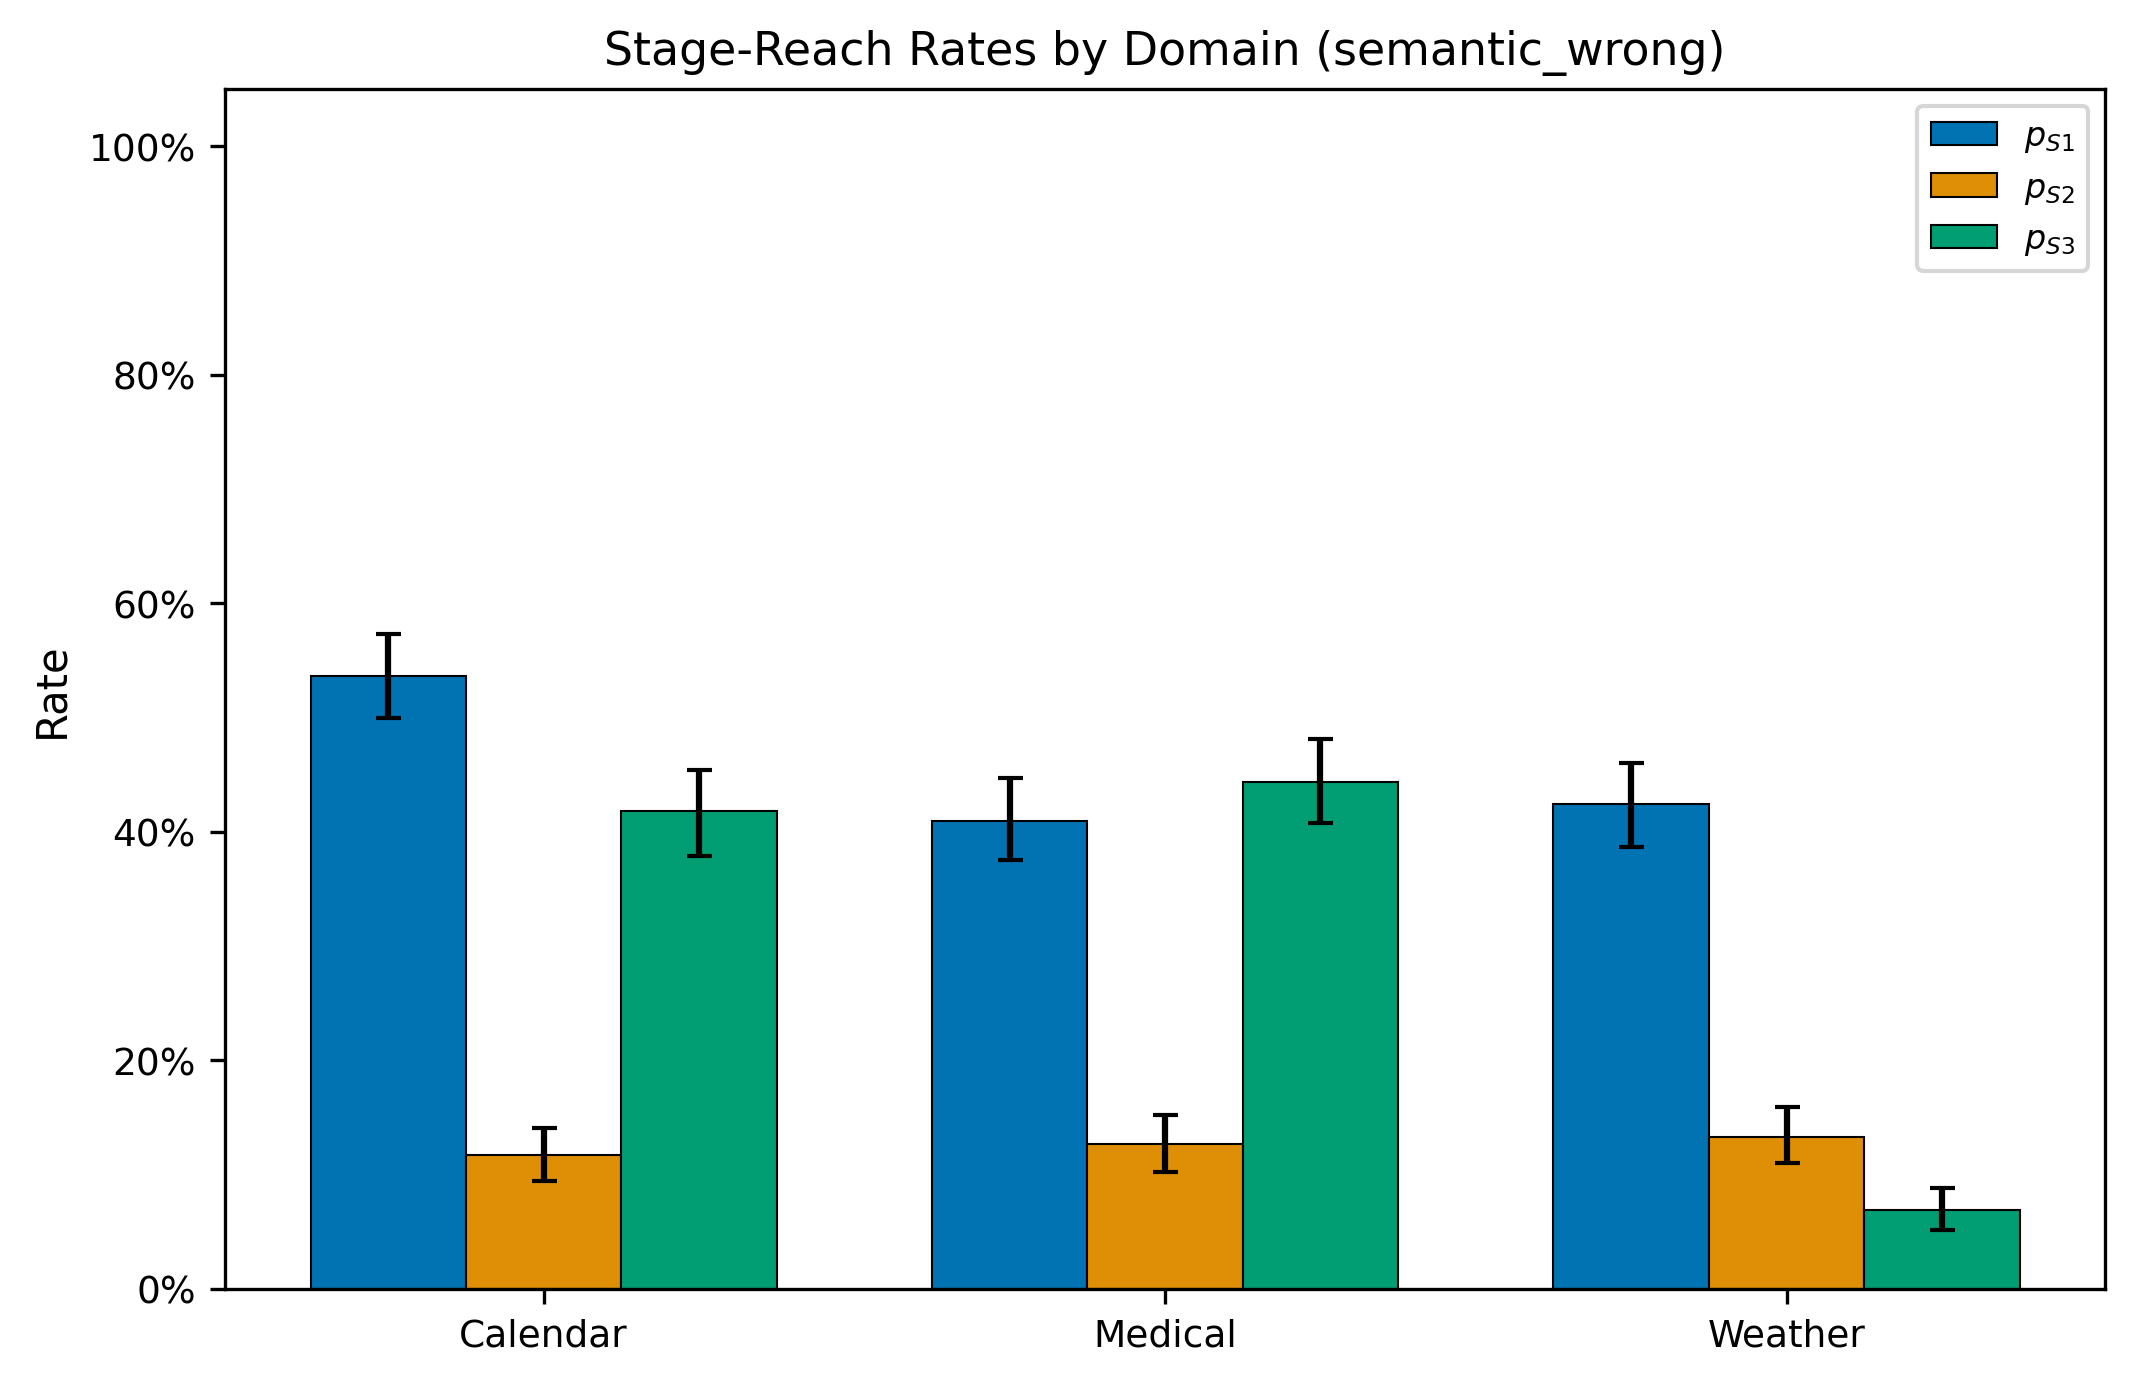
\includegraphics[width=0.8\textwidth]{figures/fig_domain_breakdown.png}
  \caption{Per-domain $S_1$, $S_2$, $S_3$ rates under P2 semantic-wrong
    injection (ensemble-judged).}
\end{figure}
\begin{figure}[h]\centering
  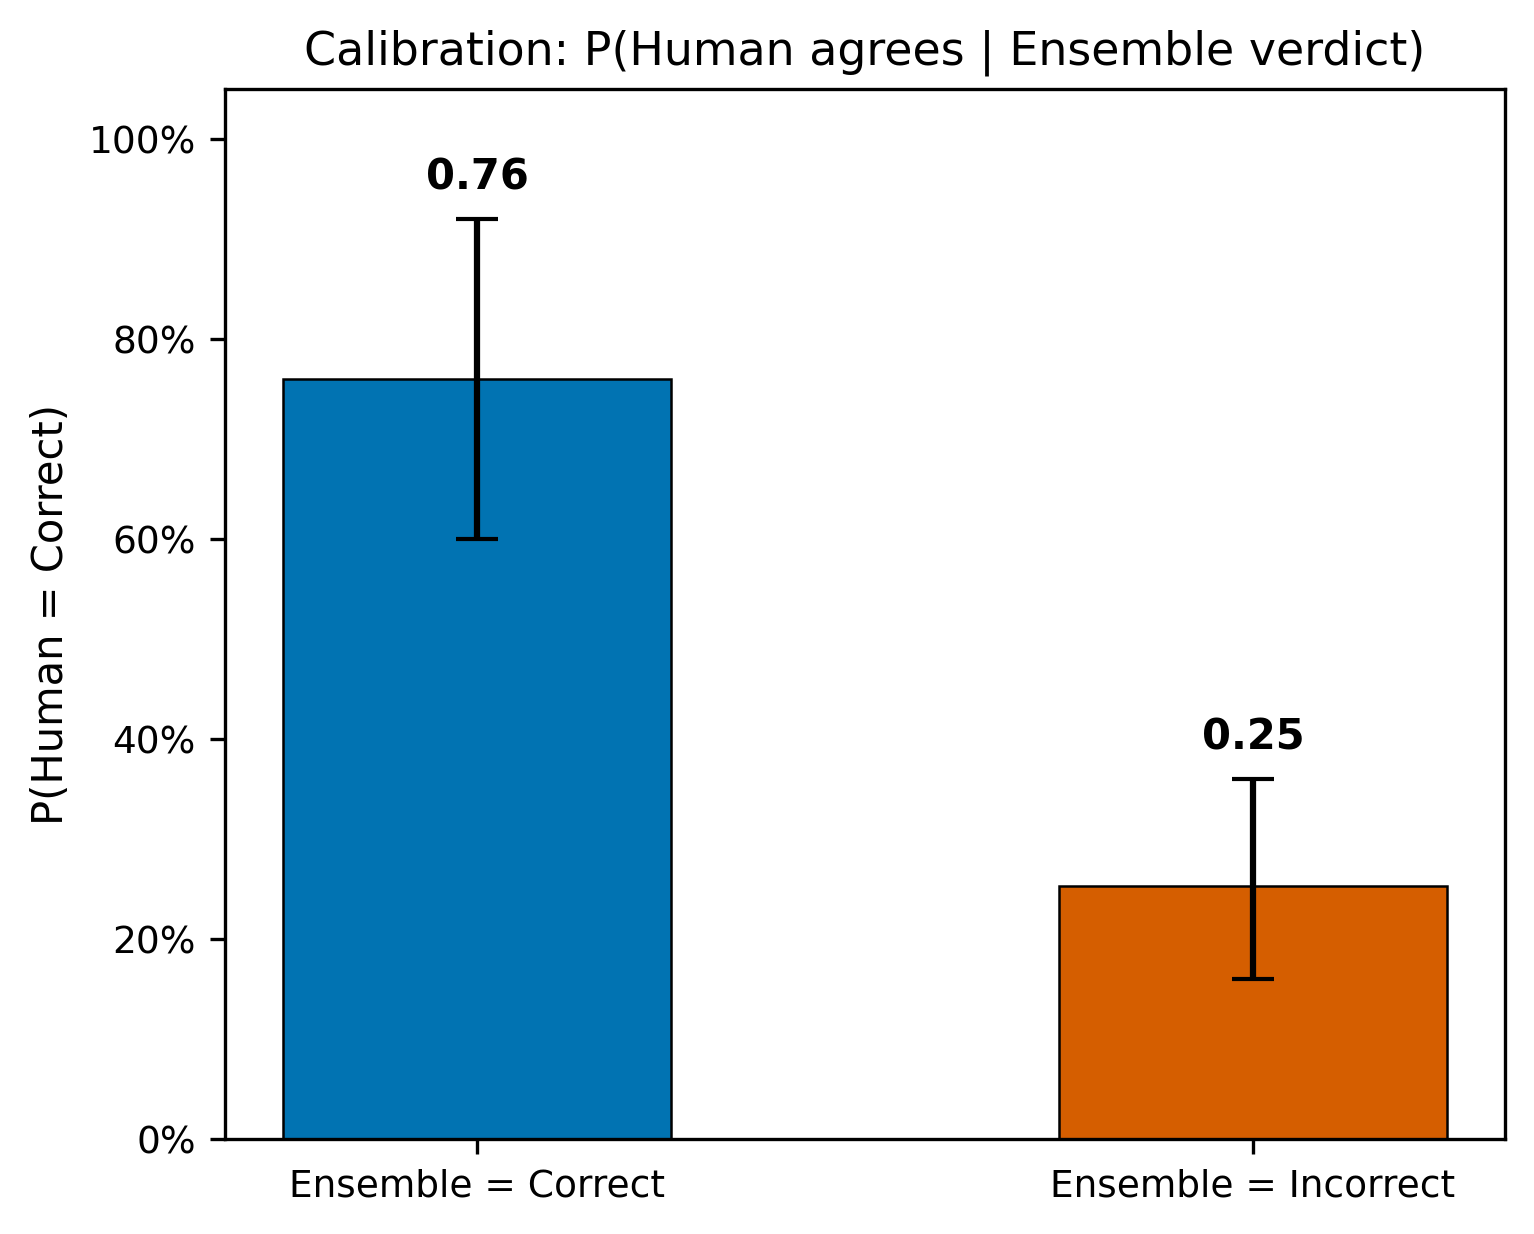
\includegraphics[width=0.6\textwidth]{figures/fig_calibration.png}
  \caption{Calibration of the ensemble judge against 100 human labels:
    $P(\text{human=correct}\mid\text{ensemble=correct}){=}0.76$;
    $P(\text{human=correct}\mid\text{ensemble=wrong}){=}0.25$.}
\end{figure}

\section{Ensemble Judge Prompt}
The identical prompt used for all three LLM judges (GPT-4o, Gemini-2.5-Flash,
GPT-4o-mini):
\begin{lstlisting}
You are an impartial judge evaluating whether an agent's final answer is correct.
QUESTION: {query}
REFERENCE ANSWER: {reference}
AGENT ANSWER: {candidate}
Respond with a single token: YES if the agent answer substantively matches the
reference, NO otherwise. Accept minor wording differences, units expressed
differently, or extra explanation as long as the core fact is correct.
YOUR VERDICT (YES or NO):
\end{lstlisting}

\section{Dataset Statistics}
\begin{table}[h]\centering
\caption{Dataset and trace statistics. P2 counts are across all four injection
types; the propagation analysis uses the semantic-wrong subset.}
\begin{tabular}{lrrl}
\toprule
Domain & Tasks & Baseline traces & Role \\
\midrule
Calendar & 667 & per model & train/eval \\
Weather  & 674 & per model & train/eval \\
Medical  & 559 & per model & train/eval \\
Knowledge & 100 & per model & ablation (no injection) \\
Retail (held-out) & 300 & 300 & cross-domain replication \\
\midrule
\multicolumn{4}{l}{\textbf{Models:} 9 proprietary + 3 open-weight (Qwen2.5
3B/7B/14B).} \\
\multicolumn{4}{l}{\textbf{Baseline traces:} 4{,}100. \textbf{P2 traces
(all types):} 9{,}400.} \\
\multicolumn{4}{l}{\textbf{Propagation analysis (semantic-wrong):} 1{,}950
across 12 models.} \\
\multicolumn{4}{l}{\textbf{Human labels:} 100. \textbf{Released agent traces:}
$>$13{,}000.} \\
\bottomrule
\end{tabular}
\end{table}

\end{document}
